% SLIDE 1: Scattering
\begin{frame}{Formación de la Imagen: Dispersión y Atenuación}
    \begin{itemize}
        \item La base de la formación de la imagen es la dispersión del haz de electrones y su posterior interferencia.
        \item Las muestras deben ser ultradelgadas para reducir la atenuación de la señal.
    \end{itemize}
    \vspace{0.5cm}
    \textbf{Regímenes de Dispersión:}
    \begin{itemize}
        \item \textbf{Señal (Elástica):} Conservación de la energía. Interacciones núcleo-electrón (alto ángulo) y nube electrónica (bajo ángulo).
        \item \textbf{Ruido (Inelástica):} Transferencia de energía a la muestra. Generación de fonones, plasmones y radiación Bremsstrahlung.
    \end{itemize}
\end{frame}

% SLIDE 2: Coherence
\begin{frame}{El Requisito de Coherencia}
    Para formar una imagen mediante interferencia y mitigar el ruido inelástico, requerimos un haz altamente coherente.
    
    \vspace{0.5cm}
    \textbf{Componentes de la Coherencia:}
    \begin{itemize}
        \item \textbf{Coherencia Espacial (Transversal):} Depende del tamaño de la fuente. Requerimos una fuente que se aproxime a un punto ideal.
        \item \textbf{Coherencia Temporal (Longitudinal):} Depende de la dispersión de energía ($\Delta E$). Vital para evitar aberraciones cromáticas exacerbadas por la dispersión inelástica.
    \end{itemize}
\end{frame}

% SLIDE 3: Electron Guns
\begin{frame}{Generación del Haz: Termiónica vs. Emisión de Campo}
    \textbf{1. Emisión Termiónica}
    \begin{itemize}
        \item \textit{Física:} Requiere altas temperaturas (degrada el material) y produce una amplia distribución de velocidades (Maxwell-Boltzmann).
        \item \textit{Modelo (Richardson-Laue-Dushman)}:
        \begin{equation*}
            J = A_G T^2 \exp{(- \Phi T^{-1})}
        \end{equation*}
    \end{itemize}
\end{frame}
\begin{frame}
    \centering
    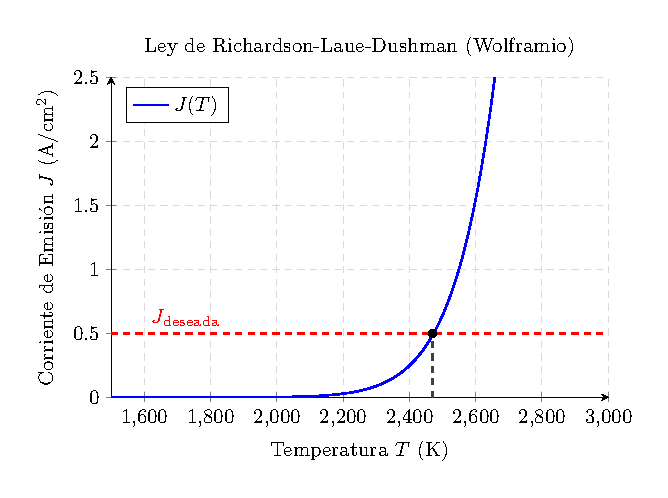
\includegraphics{emmision-current.pdf}
\end{frame}
\begin{frame}
    \textbf{2. Emisión de Campo Frío (CFEG) y Schottky}
    \begin{itemize}
        \item \textit{Física:} Un campo eléctrico deforma el potencial en una barrera triangular, permitiendo el efecto túnel cuántico.
        \item \textit{Ventaja:} Ancho de banda de energía muy estrecho ($\approx 0.3 \text{ eV}$), garantizando coherencia.
        \item \textit{Modelo (Fowler-Nordheim)}:
        \begin{equation*}
            J = A E^2 \Phi^{-1} \exp{\left(- B \Phi^{\frac{3}{2}}E^{-1}\right)}
        \end{equation*}
    \end{itemize}
\end{frame}